\documentclass[fleqn, 11pt]{article}
\usepackage{amsmath}
\usepackage{amssymb}
\usepackage{geometry}
\usepackage{graphicx}
\usepackage{bm}
\usepackage{url}
\usepackage{enumerate}
\usepackage{gensymb}
\usepackage{fullpage}
\usepackage{xcolor}

\newcommand{\Var}{\textrm{Var}}
\newcommand{\E}{\textrm{E}}

\begin{document}
\setlength\parindent{0pt}

\begin{center}
\large
\textbf{Lecture 4: Normal Distribution}\\
\normalsize
\textbf{STAT 630, Fall 2021}\\
\hrulefill
\end{center}

\begin{itemize}
\item The normal distribution is one of the most common and important probability distributions. 
\item It is symmetric, unimodal, and bell-curve shaped.
\item Many phenomena in nature follow a normal distribution such as the height of individuals, the velocity in any direction of a molecule of gas, and measurement error.
\item The normal distribution is characterized by two parameters: the mean $\mu$ (center of distribution) and standard deviation $\sigma$ (spread of distribution).
\item The notation $X \sim N(\mu,\sigma)$ means that the random variable $X$ follows a normal distribution with mean $\mu$ and standard deviation $\sigma$. 
\item For example, the plot below shows the distribution $N(\mu=10, \sigma=3)$.
\begin{figure}[ht]
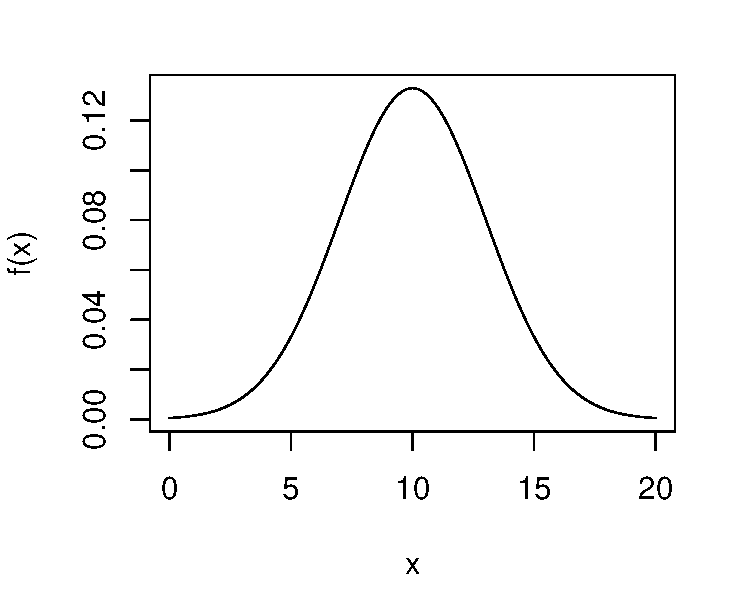
\includegraphics[scale=0.4]{figure/norm1.pdf}
\end{figure}
\item The probability density function (pdf) for the normal distribution is given by 
$$f(x) = \frac{1}{\sigma \sqrt{2 \pi}} e^{-\frac{1}{2} \left( \frac{x-\mu}{\sigma} \right) ^2}, \quad -\infty < x < \infty$$
\
\item Additional properties:
\begin{itemize}
\item The area under the normal distribution curve is 1.
$$\int_{-\infty}^{\infty} \frac{1}{\sigma \sqrt{2 \pi}} e^{-\frac{1}{2} \left( \frac{x-\mu}{\sigma} \right) ^2} dx = 1$$
\item The normal distribution is symmetric about the mean, $\mu$. 
%$P(X < \mu) = P(X > \mu) = 0.5$
\end{itemize}
\end{itemize}
\clearpage

\begin{itemize}
\item Probabilities are computed as the area under the normal distribution curve.
\begin{figure}[ht]
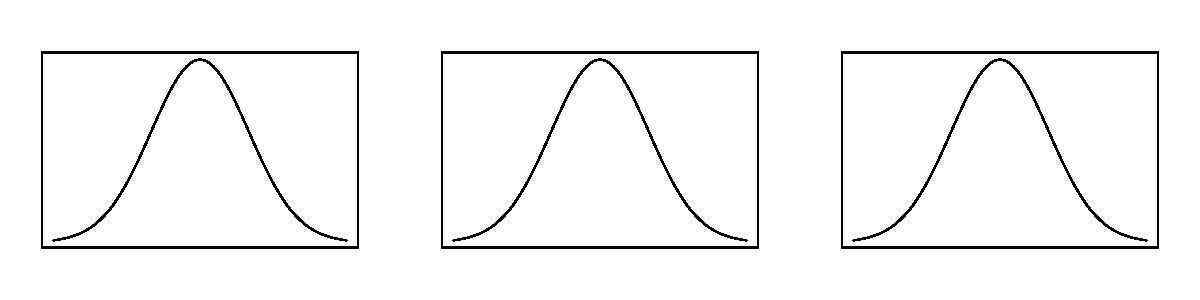
\includegraphics[width=0.95\textwidth]{figure/norm3.pdf}
% 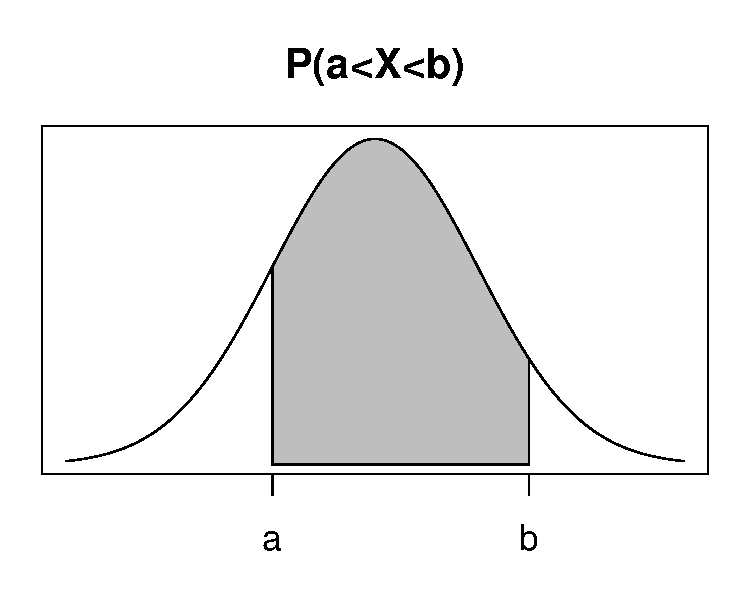
\includegraphics[scale=0.35]{figure/norm_between.pdf}
% 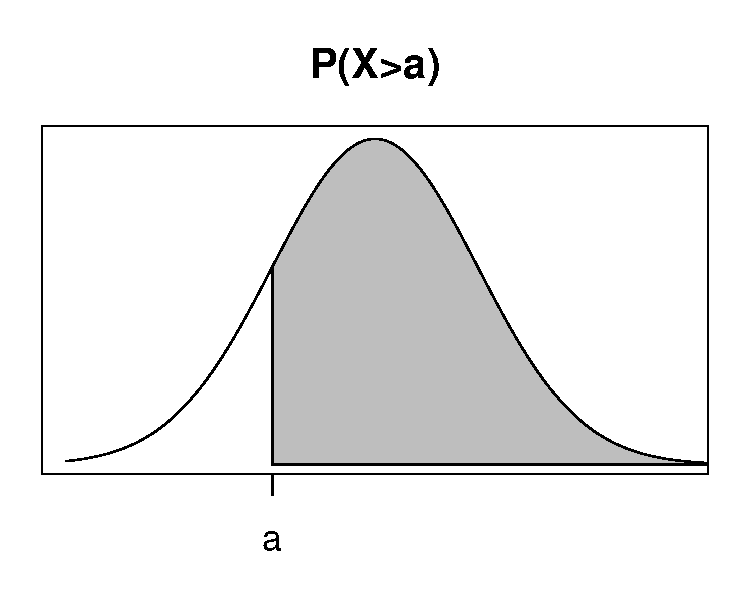
\includegraphics[scale=0.35]{figure/norm_more.pdf}
% 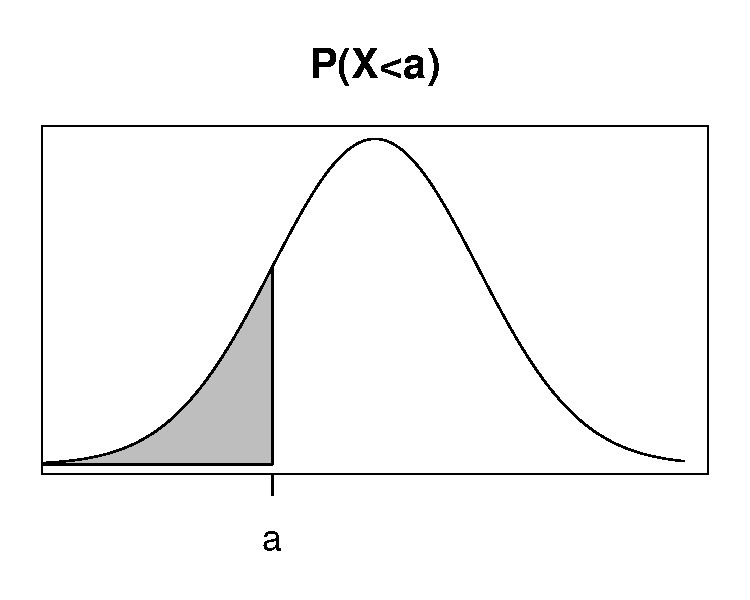
\includegraphics[scale=0.35]{figure/norm_less.pdf}
\end{figure}
\item Note that for a normally distributed random variable $P(X \geq a ) = P(X > a)$.  Why?
\vspace{35pt}
% $$ {\color{blue} P(X=a) = \int_a^a f(x) dx = 0 }$$
\item There is no closed form solution to 
$$P(X>a) = \int_a^{\infty} \frac{1}{\sigma \sqrt{2 \pi}} e^{-\frac{1}{2} \left( \frac{x-\mu}{\sigma} \right) ^2}dx,$$
so numerical approximations of the area under the curve are used to compute probabilities.  In practice, we can use the R function \texttt{pnorm()} or a standard normal table to compute probabilities.
\item Empirical Rule:
\begin{figure}[ht]
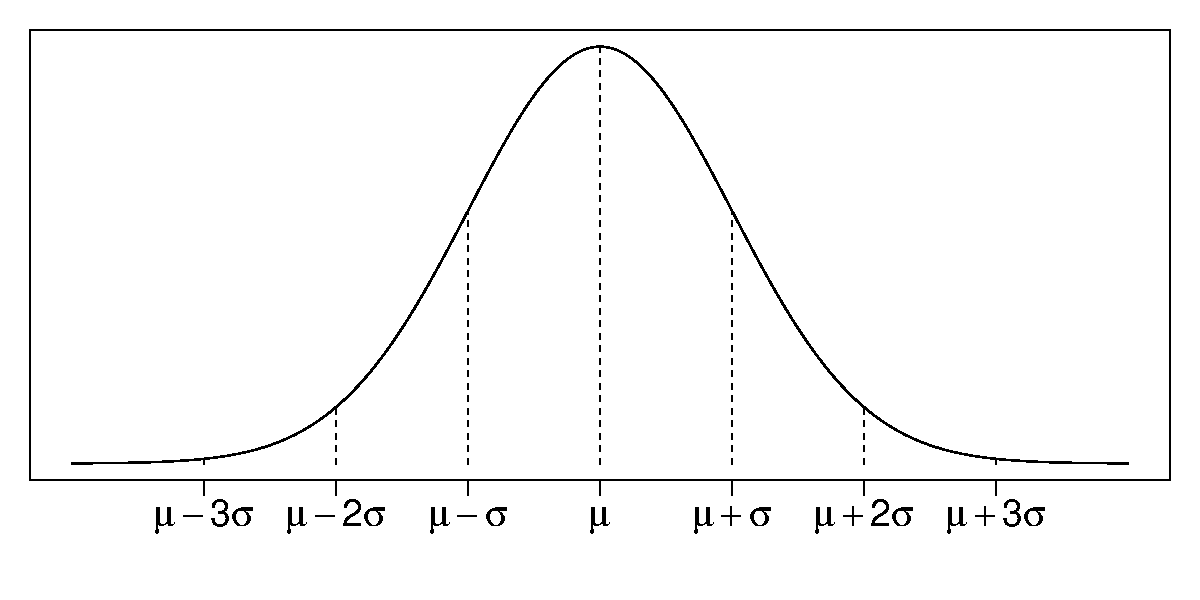
\includegraphics[scale=0.45]{figure/empirical.pdf}
\end{figure}
\begin{itemize}
\item About 68\% of the distribution is contained within 1 standard deviation of the mean.
\vspace{25pt}
% $${\color{blue} P(\mu - \sigma < X < \mu + \sigma) \approx 0.68}$$
\item About 95\% of the distribution is contained within 2 standard deviations of the mean.
\vspace{25pt}
% $${\color{blue} P(\mu - 2\sigma < X < \mu + 2\sigma) \approx 0.95 }$$
\item About 99.7\% of the distribution is contained within 3 standard deviations of the mean.
% $${\color{blue} P(\mu - 3\sigma < X < \mu + 3\sigma) \approx 0.997}$$
\end{itemize}
\end{itemize}
\clearpage


\begin{itemize}
\item Let $X \sim N(\mu, \sigma)$. A $Z$-score is defined as $Z=(X-\mu) / \sigma$.  It can be shown that $Z \sim N(0,1)$.
\item A $z$-score can be interpreted as the number of standard deviations an observation $x$ lies away from the mean.  For instance, if a student has a z-score of 2 on an exam then that student is 2 standard deviations above the average score. 
\item The distribution $N(0,1)$ is called the standard normal distribution or $Z$-distribution.
\item For $Z \sim N(0,1)$ the empirical rule gives that $P(-1 < Z < 1) \approx 0.68$, $P(-2 < Z < 2) \approx 0.95$, and $P(-3 < Z < 3) \approx 0.997$.
\item Computing $Z$-scores allows us to compute probabilities for any normal distribution.
\end{itemize}
\begin{figure}[ht]
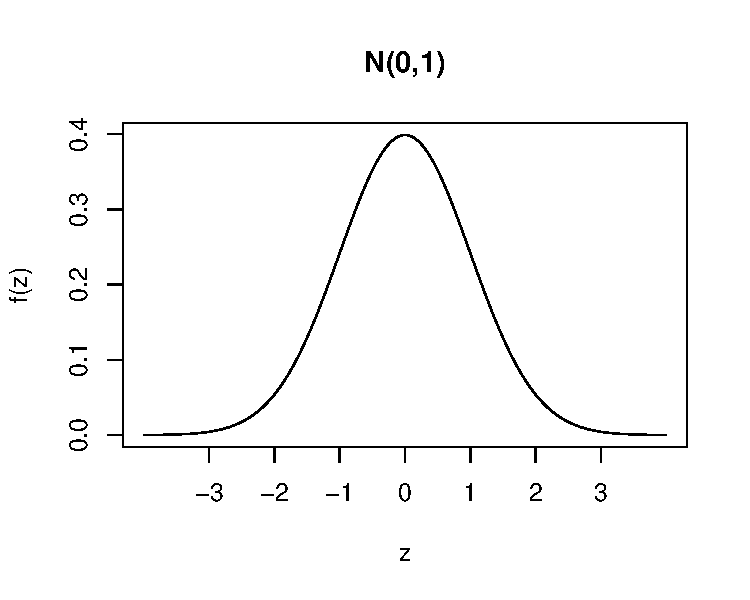
\includegraphics[scale=0.5]{figure/standnorm.pdf}
\end{figure}

\textbf{Theorem}. Let $X \sim N(\mu, \sigma)$ and $Z=(X-\mu) / \sigma$.  Show that $\E(Z) = 0$ and $\Var(Z) = 1$.\\

{\color{blue}
Properties of expectation and variance for constants $a$ and $b$:
\begin{align*}
\E(aX + b) = a \E(X) + b\\
\Var(aX + b) = a^2 \Var(X)
\end{align*}

\emph{Proof:}\\
For $Z = \frac{X-\mu}{\sigma} = \frac{1}{\sigma} X - \frac{\mu}{\sigma}$ we can let $a = \frac{1}{\sigma}$ and $b=- \frac{\mu}{\sigma}$.  It is also given that $E(X) = \mu$ and $Var(X) = \sigma^2$.  Hence,
\begin{align*}
\E(Z) &= \E\left( \frac{1}{\sigma} X - \frac{\mu}{\sigma} \right)
= \frac{1}{\sigma}\E(X) - \frac{\mu}{\sigma}
= \frac{\mu}{\sigma} - \frac{\mu}{\sigma} = 0\\
\Var(Z) &= \Var\left( \frac{1}{\sigma} X - \frac{\mu}{\sigma} \right)
= \frac{1}{\sigma^2}\Var(X)
= \frac{\sigma^2}{\sigma^2} = 1
\end{align*}
}

\clearpage
\textbf{Ex1}.  The amount $X$ of the pollutant nitrogen oxide in automobiles is normally distributed with mean $\mu=70$ ppb (parts per billion) and standard deviation $\sigma = 13$ ppb.  We can write this compactly as $X \sim N(70,13)$.
\begin{enumerate}[(a)]
\item What is the probability that a randomly selected vehicle will have an emission level less than 60 ppb?

% {\color{blue}
% \begin{align*}
%  P(X < 60) = P \left( Z < \frac{60-70}{13} \right)
% = P(Z < -0.769) = \texttt{pnorm(-0.769)} = \boxed{0.2209}
% \end{align*}
% }
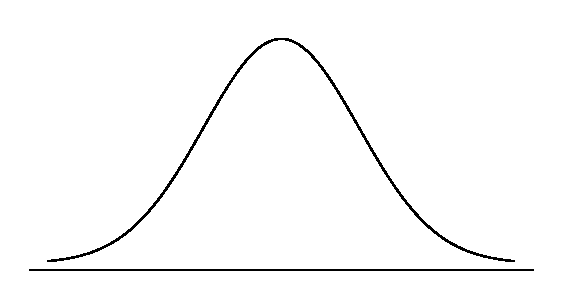
\includegraphics[scale=0.6]{figure/norm_draw.pdf}
% \bigskip
\vspace{2cm}

\item What is the probability that a randomly selected vehicle will have an emission level greater than 90 ppb?

% {\color{blue}
% \begin{align*}
% P(X > 90) &= P \left( Z > \frac{90-70}{13} \right)
% = P(Z > 1.538) = 1 - P(Z < 1.538)\\ 
% &= \texttt{1 - pnorm(1.538)} = \boxed{0.062}
% \end{align*}
% }
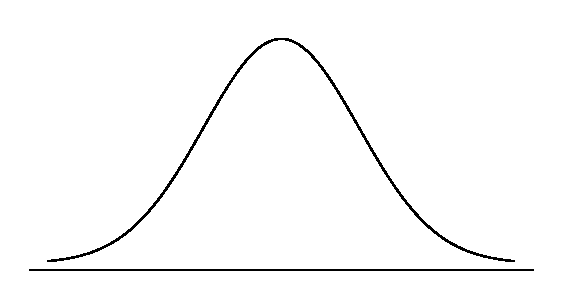
\includegraphics[scale=0.6]{figure/norm_draw.pdf}
% \bigskip
\vspace{2cm}

\item What is the probability that a randomly selected vehicle will have an emission level between 60 and 90 ppb?

% {\color{blue}
% \begin{align*}
% P(60 < X < 90) &= P(X < 90) - P(X < 60)\\ 
% &= P \left( Z < \frac{90-70}{13} \right) - P \left( Z < \frac{60-70}{13} \right)\\
% &= P(Z < 1.538) - P(Z < -0.769)\\
% &= \texttt{pnorm(1.538) - pnorm(-0.769)}
% = \boxed{0.717}
% \end{align*}
% }
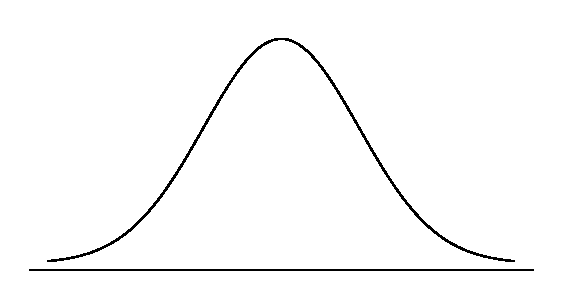
\includegraphics[scale=0.6]{figure/norm_draw.pdf}
\end{enumerate}  
\clearpage

\textbf{Ex2}.  Body temperatures are normally distributed with mean $\mu=98.2$ and standard deviation $\sigma= 0.74$, in degrees Fahrenheit.  That is, $X \sim N(98.2, 0.74)$.  
\begin{enumerate}[(a)]
\item Find the cutoff for the lowest 5\% of body temperatures (the $5^{th}$ percentile)?\\

{\color{blue}
$X \sim N(98.2, 0.74)$; want to find $5^{th}$ percentile.\\

In R, $\texttt{qnorm(0.05) = -1.645}$ gives the $0.05$ quantile of the standard normal distribution.  So, $P(Z < -1.645) = 0.05$.  Next, solve for $x$ in the equation for a $z$-score:
\begin{align*}
z = \frac{x - \mu}{\sigma} \implies
-1.645 = \frac{x - 98.2}{0.74} \implies
x = (-1.645)(0.74) + 98.2 = \boxed{96.983}
\end{align*}
}
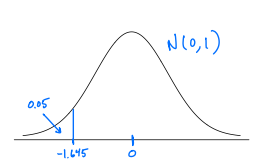
\includegraphics[scale=0.65]{figure/2a.png}
\bigskip
% \vspace{6cm}

\item Find the cutoff for the highest 15\% of body temperatures (the 85$^{th}$ percentile)?\\

{\color{blue}
$X \sim N(98.2, 0.74)$; want to find $85^{th}$ percentile.
\medskip

In R, \texttt{qnorm(0.85) = 1.036} gives the 0.85 quantile of the standard normal distribution. So, $P(Z < 1.036) = 0.85$.  Next, solve for $x$ in the equation for a $z$-score:
\begin{align*}
z = \frac{x - \mu}{\sigma} \implies
1.036 = \frac{x - 98.2}{0.74} \implies
x = (1.036)(0.74) + 98.2 = \boxed{98.967}
\end{align*}
}

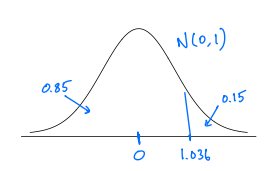
\includegraphics[scale=0.67]{figure/2b.png}
\end{enumerate}
  





 
\end{document}